\chapter{Background}

\section{Cumulus Clouds}
\subsection{What is cumulus clouds?}

\begin{figure}[htp]
\begin{center}
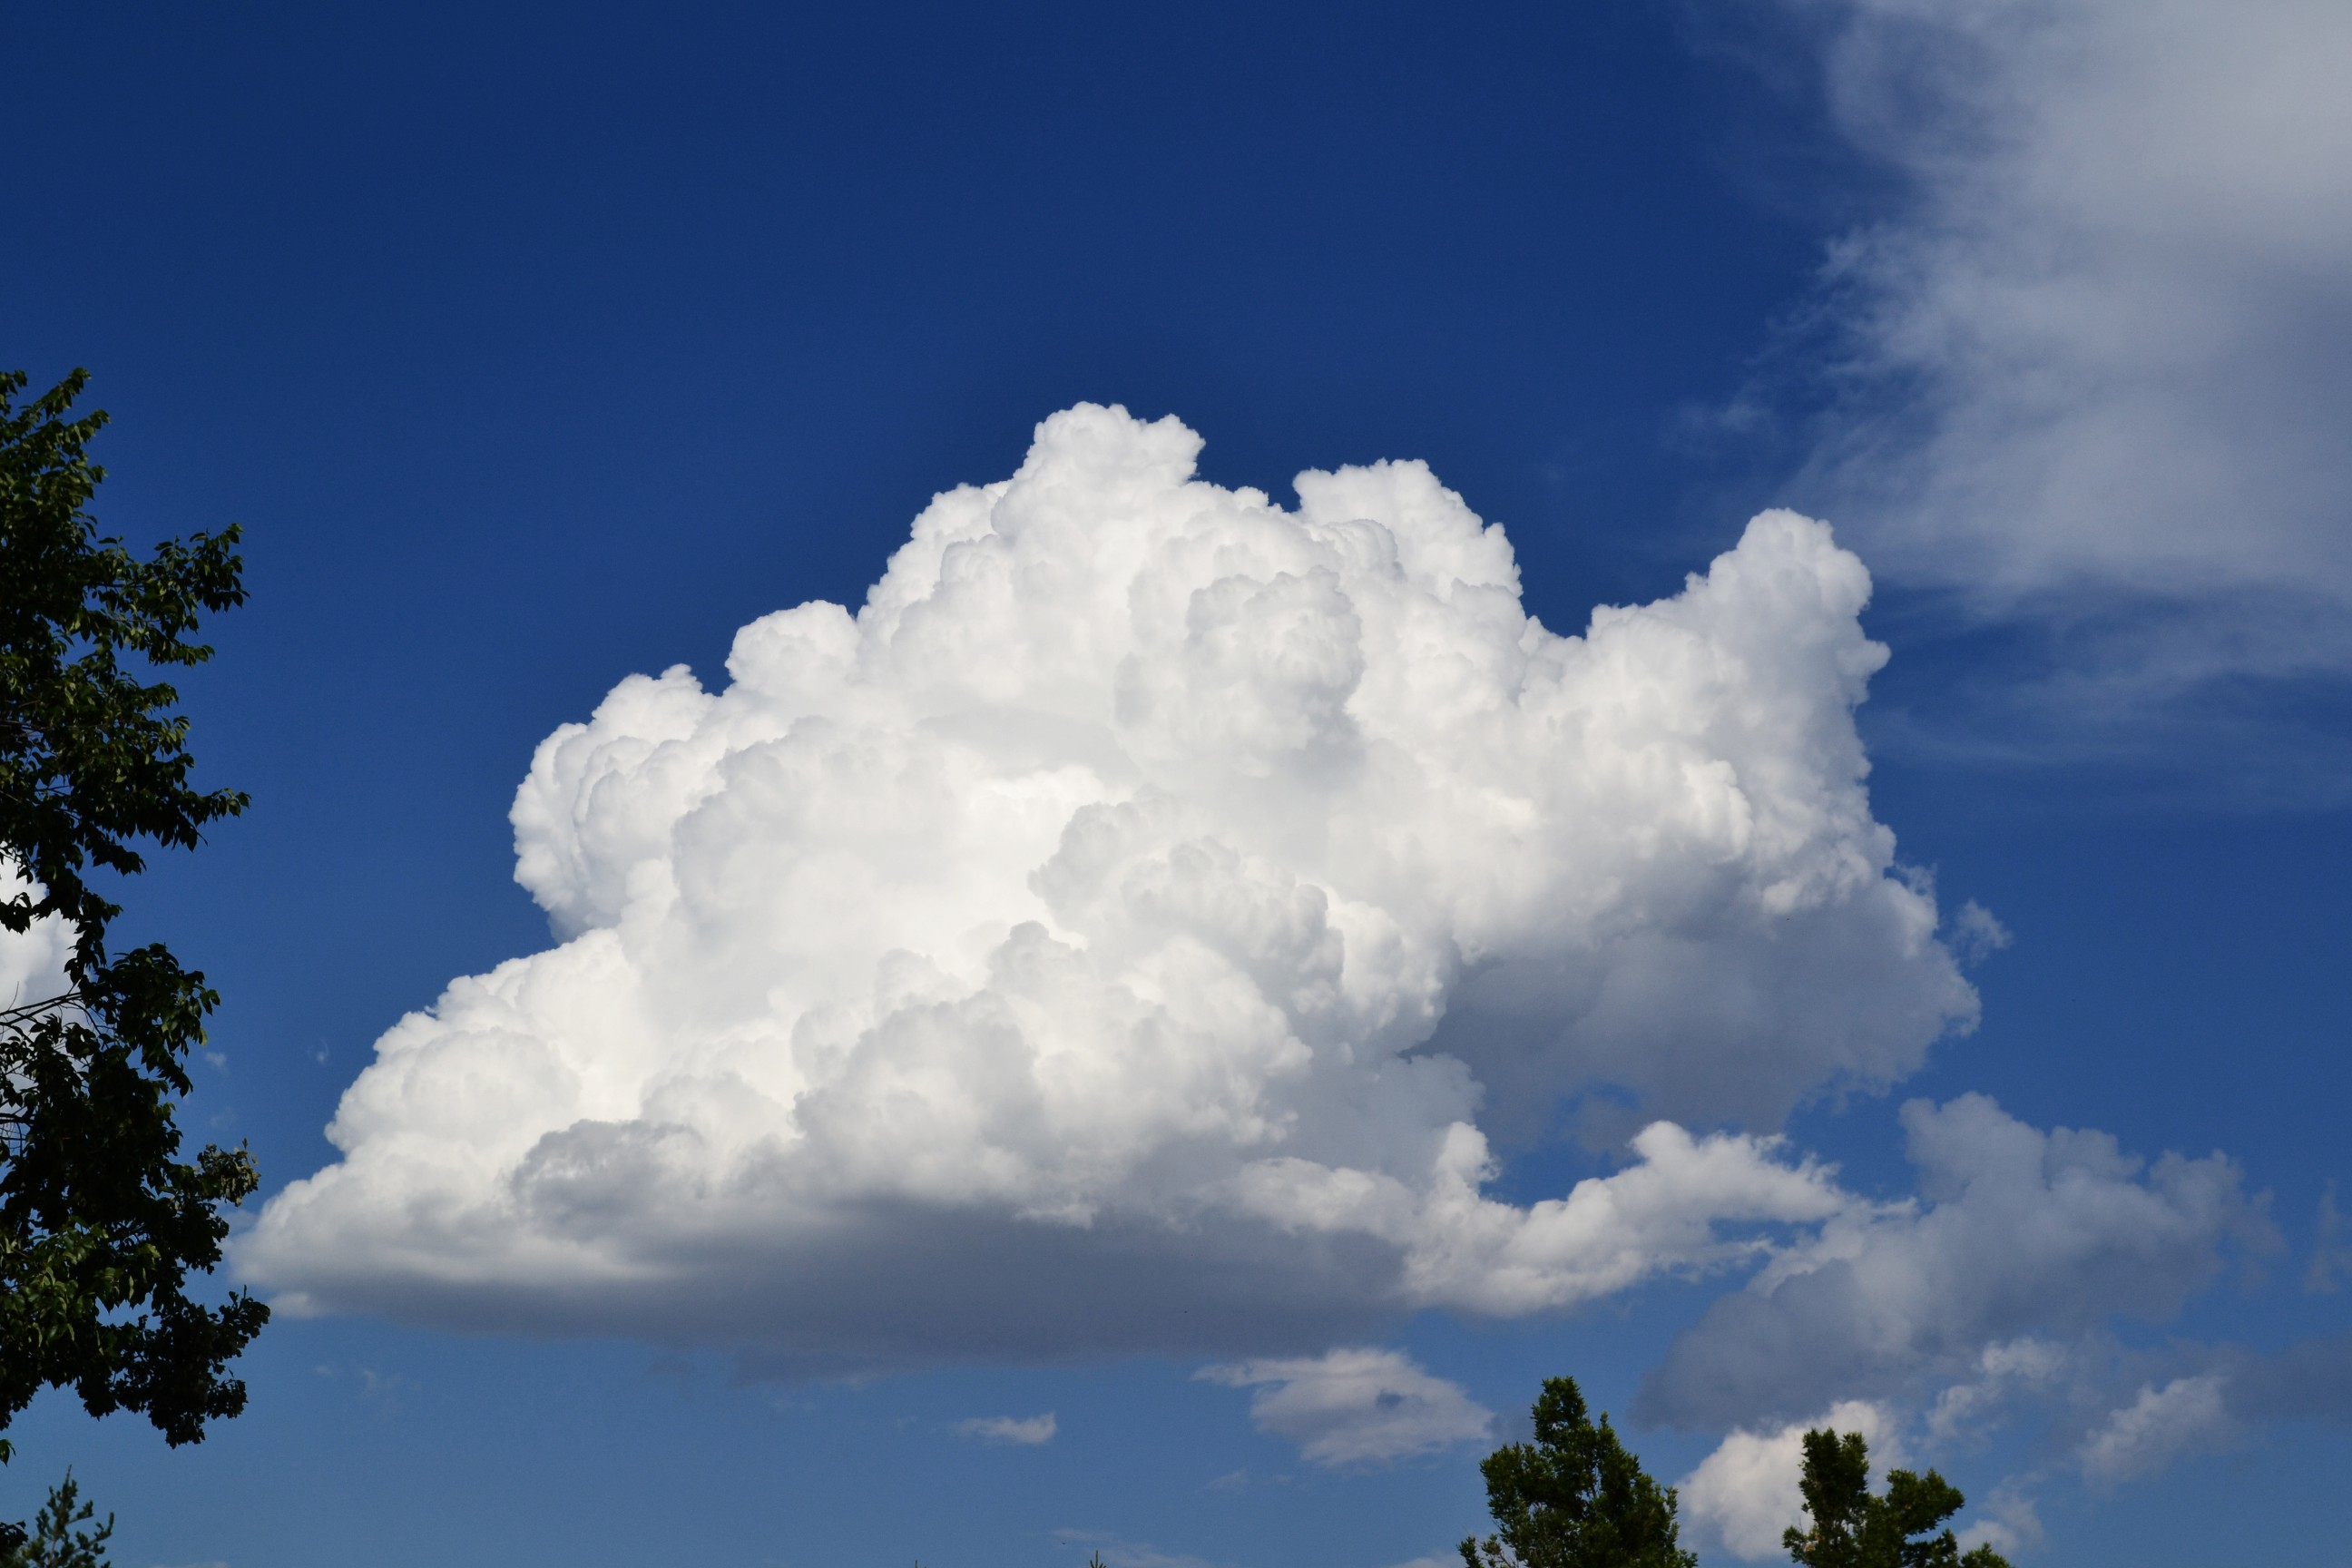
\includegraphics[scale=0.13]{images/single-fluffy-cumulus-cloud-sunny-day-2012-07-26.jpg}
\caption{Single cumulus cloud}
\label{f1}
\end{center}
\end{figure}

Cumulus clouds are a genus-type of low-level cloud that can have noticeable vertical development and clearly defined edges. Cumulo- means "heap" or "pile" in Latin. They are often described as "puffy" or "cotton-like" in appearance, and generally have flat bases. Cumulus clouds, being low-stage clouds, are generally less than 3,300 ft in altitude unless they are the more vertical cumulus congestus form. Cumulus clouds may appear by themselves, in lines, or in clusters.

\subsection{Why does the paper concentrate on rendering cumulus clouds?}
Among the numerous kinds of clouds in the nature environment, cumulus clouds have the most pronounced volumetric feature, making the volumetric rendering more practical. In the final step of the proposed method from the paper, a volume-aware blending is performed. If we use other kind of clouds, such as stratus clouds or cirrus clouds, the volumetric feature can be hardly found, which is not able to be rendered as physically based clouds. This is because we will need a volume to calculate the light occlusion later on.

\section{Existing Method to render clouds in real time}
Off-line rendering can be quite accurate about simulating the cloud, but it could take minutes to hours to draw a single frame. We'll be looking into the existing real time rendering methods in the following subsections.

\subsection{Billboards}
